\chapter{面向全网络高级SDN程序的数据平面实现问题的研究}

\section{引言}

随着SDN技术的广泛应用以及底层可编程数据平面技术的不断发展(即从单流表到多流表流水线到自定义多流表流水线),如何实现面向全网络(即多交换机)可编程数据平面的高级SDN编程变得越来越重要。具体来说,我们需要达到,在保持高级SDN编程模型的同时,用户编写的高级SDN程序通过系统可以自动地编译成多个可编程数据通路的配置。

与传统SDN技术相比较,通过自定义多流表流水线技术(例如,P4~\cite{P4}),可编程数据通路的配置需要包括自定义的流水线结构,以及相应的流表内容。而在传统SDN中,由于只考虑单流表的数据平面(或具有特定功能的数据平面),其配置只包括流表内容。例如,Maple~\cite{voellmy2013maple}通过控制器上收到的数据包,建立踪迹树的结构,并生成流表规则。但它并没有主动地生成流表规则,并且只考虑了单流表结构。Beckett等人~\cite{beckett2016don}利用领域特定语言,让用户可以表达BGP上的目标以及约束,并最终生成每个交换机的配置。但他们考虑的是特定的网络场景(即BGP)。Tian等人~\cite{tian2019safely}通过意图模型,自动地生成了ACL(Access Control List)中的规则,并且实现了自动更新。但他们只考虑了特定的网络功能(即ACL)。

在面向全网络的可编程数据通路自动配置的工作中,Arashloo等人~\cite{snap}考虑有状态交换机,并将高级SDN程序自动地编译为多个有状态交换机的配置。但其基于的是One-Big-Switch模型,用户在编程时只可以看到终端主机,而没有网络拓扑细节信息(即相当于一个大的交换机)。因此用户无法让数据包沿着特定的路径进行转发。

本章中,我们将考虑基于多交换机的高级SDN程序数据平面实现问题。对于数据平面,我们分为两大类:完全可编程网络以及部分可编程网络。完全可编程网络是指,网络中的交换机均支持可配置的数据通路(如P4)。而部分可编程网络是指,网络中不光包含支持可配置的数据通路,并且包含只可以实现特定功能的中间盒(如防火墙等)。对于上述两类数据平面,我们都要考虑高级SDN程序的实现问题。

\section{完全可编程网络实现问题}

我们考虑的面向全网络SDN编程模型本质上与单交换机的编程模型类似,同样参考已有的SDN编程模型(如~\cite{snap,sivaraman2016packet})。但面向全网络的SDN程序的返回则是网络中的一条路径(即多个交换机的操作),而非单个交换机的操作。因此,对于程序的返回,我们采用路由代数的形式进行表达~\cite{gao2018t}。我们通过以下示例程序进行说明。

\begin{figure}[h]
\small{
\begin{verbatim}
L1: def onPkt(pkt):
L2:   if pkt.srcIP in whiteList:
L3:     srcHost = hostTable(pkt.srcIP)
L4:     dstHost = hostTable(pkt.dstIP)
L5:     if pkt.dstPort in portList:
L6:       return opt(srcHost -> dstHost)
L7:     else:
L8:      return opt(srcHost -> c -> dstHost)
L9:   else: return DROP
\end{verbatim}
}
    \caption{\small 一个简单的面向全网络的高级SDN程序。}
\label{fig:code1}
\end{figure}

如图~\ref{fig:topo1}所示,用户希望对于目的端口不在\emph{portList}的数据流必须经过节点$c$(程序中L5-L8)。并且源IP不在\emph{whiteList}的数据包进行丢弃(程序中L2)。程序的返回为路由代数,如程序中的L6和L8分别表示\emph{srcHost}到\emph{dstHost}的最优路径(即最小跳数),\emph{srcHost}到\emph{dstHost}并经过$c$的最优路径。

\begin{figure}[!htbp]
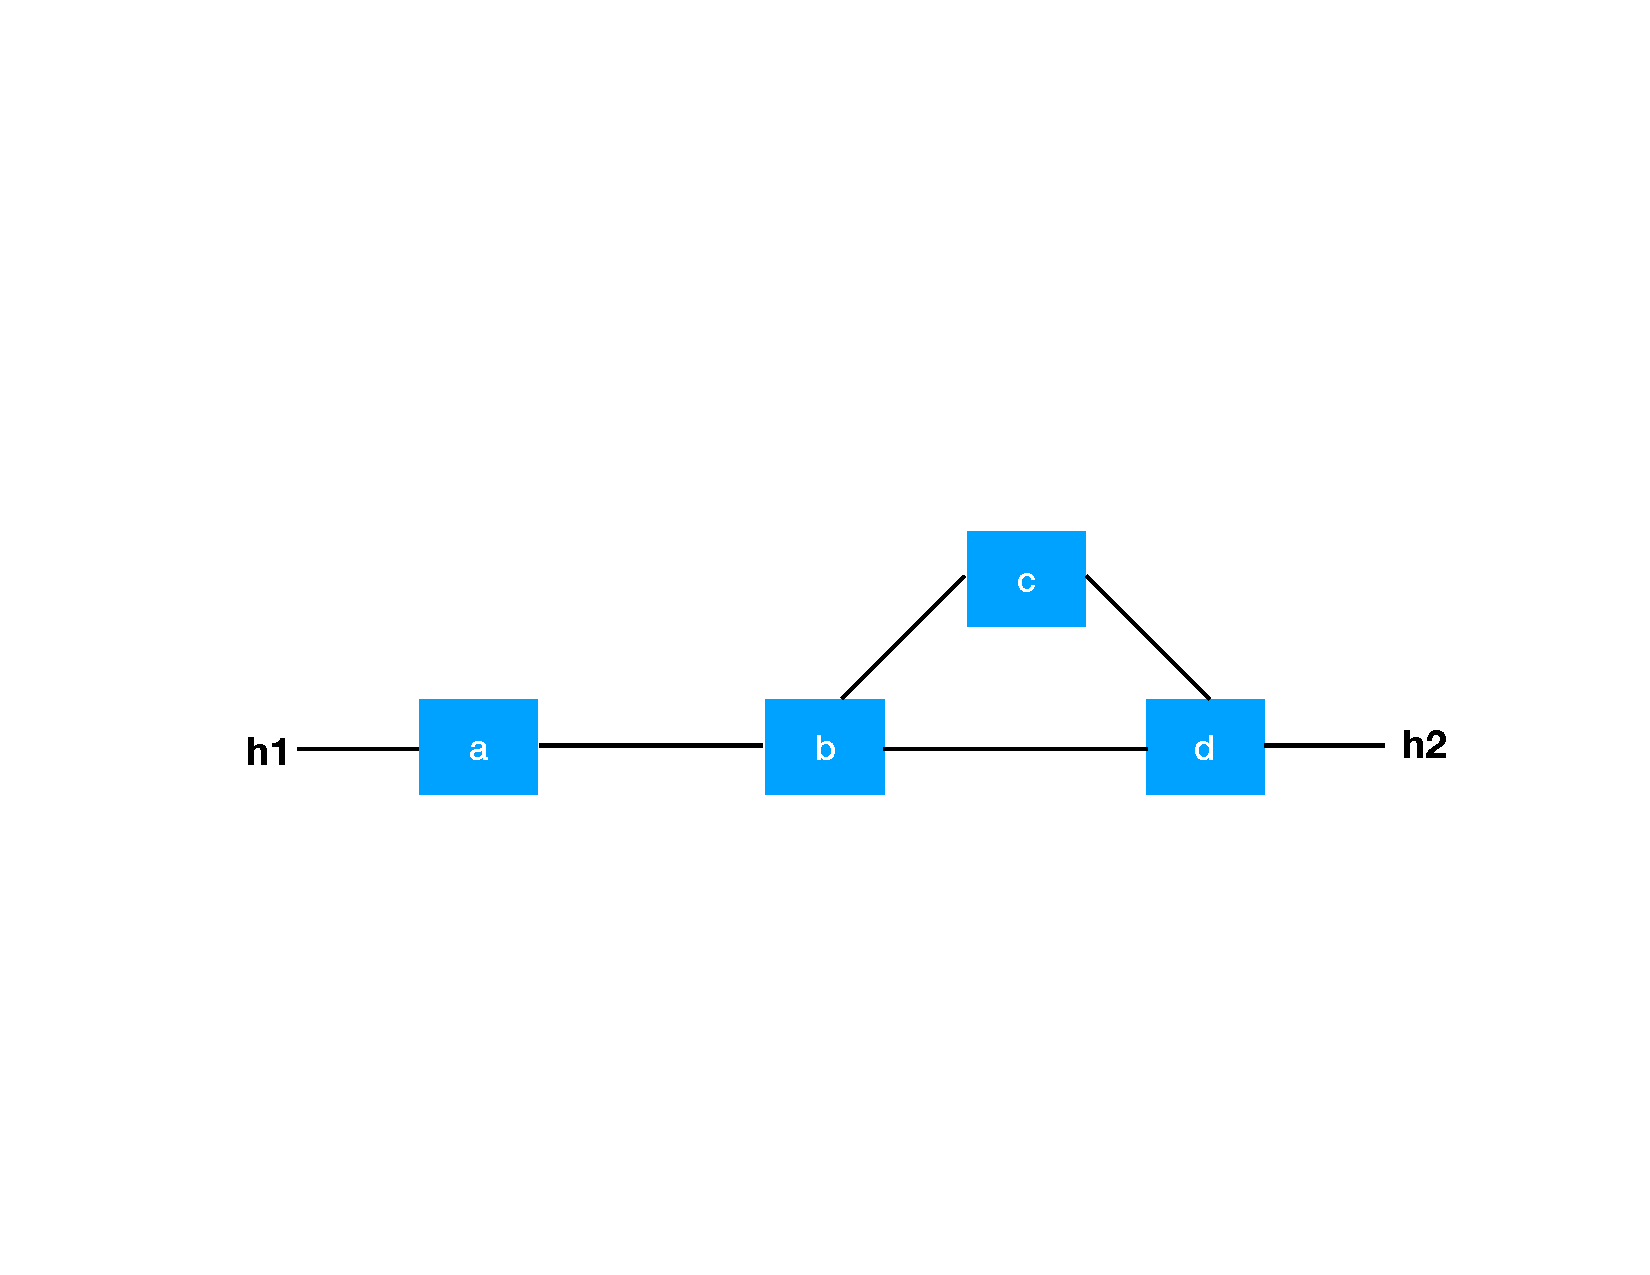
\includegraphics[width=0.8\linewidth]{figures/global-topo.pdf}
\centering
\caption{\small 本节示例程序对应的网络拓扑。}
\label{fig:topo1}
\end{figure}

对于完全可编程网络,在不考虑交换机资源限制情况下,当一个高级SDN程序除了返回路径的语句之外都可以在单交换机上实现时,该程序也可以非常简单地在该完全可编程网络中实现。实现方法如下:将程序的所有逻辑放到边缘交换机,并通过封装数据包的方式,使数据包穿越网络。如图~\ref{fig:topo1}所示,边缘交换机为连接着主机的交换机$a$和$d$,因此可以把程序的逻辑全部放在$a$和$d$上。然而当网络资源有限时(即边缘交换机流表资源不够,无法实现程序的全部逻辑),该方法是不对的。

当资源受限时,我们的目标则是将程序``打散",使其不同部分实现在不同交换机上。然而,确定哪些部分实现在哪些交换机上是一个问题。SNAP考虑了类似的问题,由于其依赖于One-Big-Switch模型,SNAP并不支持用户程序自定义的路径。而自定义路径会使问题变得复杂。如图~\ref{fig:topo1}所示,对于$h2$发往$h1$的数据流,由于交换机$d$需要判断数据包的目的端口,因此$d$必须包含程序的全部逻辑。当网络以及程序变得复杂时,我们需要一个方法将程序实现在网络中。



\para{程序的决策树}:我们首先对程序生成决策树。决策树的每一个内部节点为程序的一个语句;叶子节点为程序返回的路径。图~\ref{fig:dg}给出了示例程序的部分决策树。决策树生成的一种做法是符号执行~\cite{king1976symbolic},Voellmy等人~\cite{magellan-poster}给出了相应的做法,因此我们这里不对如何生成决策树进行展开。

\begin{figure}[!htbp]
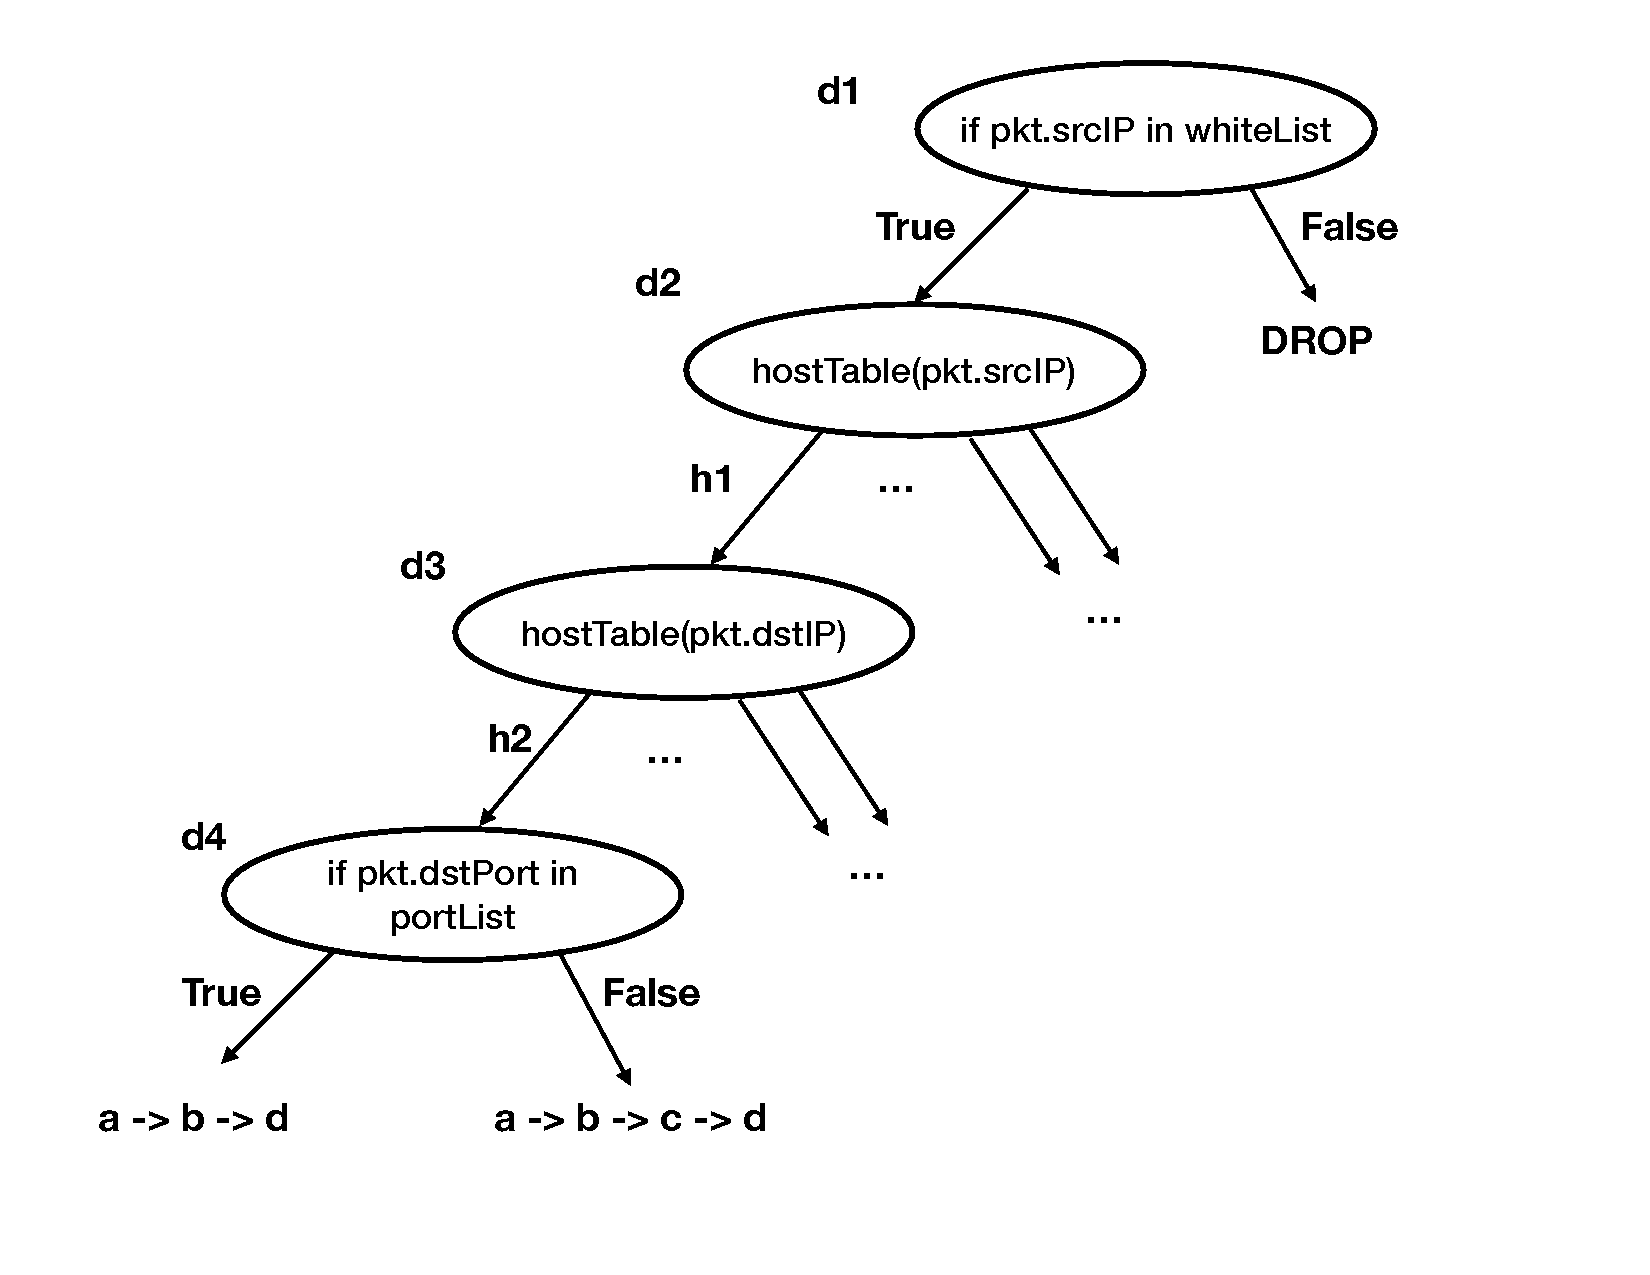
\includegraphics[width=0.8\linewidth]{figures/global-dt.pdf}
\centering
\caption{\small SDN程序对应的决策树。}
\label{fig:dg}
\end{figure}

基于决策树,我们现在可以判断哪些语句必须要在一些交换机上执行。做法如下:从每个边缘交换机开始考虑。对于边缘交换机$n$,若决策树的叶子节点中的路径的初始节点不是$n$,则删除该叶子节点以及相应的无效边。然后从根节点开始计算所有内部节点(包括根节点)下面的叶子节点中路径的下一跳交换机,并将其标识在内部节点上(称为该节点可能的下一跳)。若一个节点可能的下一跳都相同,则说明该节点对应的语句可以在后面执行。因此,基于所有节点可能的下一跳,我们可以得到哪些语句一定要在该边缘交换机上执行。对于其余节点,则沿着同样的下一跳,在下一个交换机执行相同过程(在此之前从所有叶子节点的路径中删除$n$)。最终,我们可以得到:对所有路径上的所有需要执行的语句,它们都有相应的可执行交换机的范围。

\para{示例}:考虑图~\ref{fig:dg}中的决策树。我们发现对于边缘交换机$a$,决策树上的所有节点的可能的下一跳都相同($b$)。因此,所有的语句可以不在$a$上执行。当整个决策树移到$b$时(此时叶子节点已经被更新),我们发现所有的节点的可能的下一跳都不同(均为$c$或$d$)。因此,我们得到所有语句的可以执行的范围为交换机$a$或$b$。


在确定每个语句(决策树上内部节点)可以执行的交换机范围后,我们可以通过混合整数线性规划进行求解。其中变量在表~\ref{table:variables}给出;约束在表~\ref{table:constraints}给出。系统的目标可以是:minimize $max(\sum_{d_j^i} x(d_j^i, n))$,即最小化所有交换机最多实现的语句数量,使程序语句可以相对均匀地分布在网络中。

最终,通过计算混合整数线性规划,我们可以得到决策树中节点与网络交换机的对应关系,即对于每个交换机,我们可以得到它应该实现哪些程序语句,进而算出交换机配置。

\begin{table}[]
\centering
\begin{tabular}{l|l}
\hline
变量     & 含义                                                             \\ \hline
$p_i$ & 转发路径$i$,包含一串有序的网络节点以及一串有序的决策树节点                            \\ 
$n_j^i$          &  $p_i$中第$j$个网络节点                      \\
$d_j^i$        & $p_i$中第$j$个决策树节点                                            \\
$code_i(n)$        &  网络节点$n$对于$p_i$的编号\\
$N_j^i$     &  $d_j^i$可以选择的网络节点的集合\\
$x(d_j^i, n)$      &  1: $d_j^i$选中网络节点$n$; 0: $d_j^i$未选中网络节点$n$\\
$m(n)$              & 网络节点$n$最多可以实现的决策树节点数量\\
\hline              
\end{tabular}
\caption{\small 本节线性规划所用的变量。}
\label{table:variables}
\end{table}

\begin{table}[]
\centering
\begin{tabular}{l|l}
\hline
约束                                        & 含义                               \\ \hline
$xc_j^i = \sum_n x(d_j^i, n)*code_i(n)$          & 决策树节点选中的网络节点的编号   \\
$\forall d_j^i, xc_j^i \leq xc_j^{i+1}$                    & 保证决策树节点之间的依赖关系                  \\
$\forall d_j^i, \exists n \in N_j^i, xc_j^i = code_i(n)$      & 对决策树节点可选的网络节点的范围进行约束     \\
$\forall n, \sum_{d_j^i} x(d_j^i, n) \leq m(n)$   & 保证网络节点资源 \\
$\forall d_j^i \sum_n x(d_j^i, n) = 1$  & 保证决策树节点与网络节点的一对一映射\\
\hline
\end{tabular}
\caption{\small 本节线性规划所用的约束。}
\label{table:constraints}
\end{table}


\section{部分可编程网络实现问题}

与完全可编程网络相比,部分可编程网络中包含具有特定、固定功能网络节点,如中间盒等。而程序可以利用这些网络节点的功能对数据包进行处理。

首先给出我们设计的使用户能指定网络中的中间盒的原语。第一个是指定网络中的中间盒,\codeword{m = middlebox(name, property)}。其中property标识该中间盒是否有状态。第二个是调用中间盒对数据包的处理,\codeword{m.handle(pkt)}。具体来说,我们考虑一个中间盒为一个数据包处理函数。它可以返回对收到的数据包进行处理的结果。对于一个无状态中间盒,如果两个数据包具有相同的五元组,则它们的返回结果也相同;对于一个有状态中间盒,由于数据包的处理会考虑中间盒的状态,即使两个数据包具有相同的五元组,它们的返回结果也不一定相同。

除了中间盒原语之外,为了让用户指定数据包在网络传输的路径的约束,这里也引入了路由代数作为程序的返回。图~\ref{fig:grammar2}给出了对于部分可编程网络编程模型的抽象语法。对于中间盒,编程人员可以指定其属性,即有状态或无状态。中间盒的返回结果可以存储在一般变量中,在接下来的程序中调用。

\begin{figure}[ht]
{\small
% \fontsize{10}{12}\selectfont 
%\scriptsize
%{\bf Abstract syntax:}
%\vspace{-2mm}
\[%\arraycolsep=1.4pt\def\arraystretch{2.2}
\begin{array}{rclr}
p &\bnfdef & \ONPKT\ \{I\},\ d_1,\ \ldots,\ d_n &(\textit{program})\\
d &\bnfdef & x^r\ =\ r\  & (\textit{route algebra decl})\\
 & & \bnfalt x^m\ =\ middlebox(n,\ s) & (\textit{middlebox decl})\\
I &\bnfdef & x\ =\ e & \\
 & & \bnfalt I;I &  (\textit{sequencing})\\
 & & \bnfalt x\ =\ x^m.handle(pkt) &  (\textit{middlebox operation})\\
 & & \bnfalt \ifelse{e^b}{I}{I} &  (\textit{conditional})\\ %\\ 
 & & \bnfalt \return{x^r} \bnfalt \return{r} &  (\textit{func return})\\ 
% & & \bnfalt m[e_1, \dots, e_n] := e & (\textit{map update}) \\
% & & \bnfalt s := s \cup \{e\} \bnfalt s := s - \{e\} & (\textit{set update}) \\
e &\bnfdef & c \bnfalt x &  (\textit{consts, vars})\\
%& & \bnfalt x^r  & (\textit{route algebra vars}) \\
& & \bnfalt x^m & (\textit{middlebox vars}) \\
& & \bnfalt pkt.a & (\textit{packet fields}) \\
% & & \bnfalt e+e \bnfalt e*e \dots & (\textit{arith}) \\ 
e^r & \bnfdef & e == e \bnfalt e \leq e \dots & (\textit{relational})\\
e^b & \bnfdef & e^r \bnfalt e^r\ \&\ e^r \bnfalt e^r\ |\ e^r \dots & (\textit{boolean})\\
(r &{\color{blue}{\in}}&\mathit{route\ algebra\ expressions}) & \\
(c &{\color{blue}{\in}}& \mathit{strings}) & (\mathit{consts})\\
(a &{\color{blue}{\in}}& \{ \mathit{macSrc}, \mathit{ipDst} \dots \}) & (\textit{packet fields})\\
(n &{\color{blue}{\in}}& \mathit{strings})  &  (\textit{middlebox names})\\
(s &{\color{blue}{\in}}& \{ \mathit{stateless},\mathit{stateful} \})  &  (\textit{properties})\\
(x &{\color{blue}{\in}} & \{\tx_1,\tx_2,\dots,\ty_1,\dots\}) &  (\textit{variables})\\
\end{array}\]}% small
%\vspace{1mm}
% \hrule
%\vspace{-5mm}
\caption{引入中间盒处理的抽象语法。}
\label{fig:grammar2}
\end{figure}

\para{示例}:基于图~\ref{fig:grammar2}给出的抽象语法,我们考虑如下引入了中间盒处理的高级SDN程序。同时网络场景为图~\ref{fig:topo2}所示。

\begin{figure}[h]
{\small
\begin{verbatim}
L1: mFW = middlebox("firewall", "stateless")
L2: PATH1 = h1 -> b -> h2 //b: waypoint
L3: PATH2 = h1 -> c -> h2 //c: waypoint
L4: //any: picking any path
L5: def onPacket(pkt):
L6:   if pkt.srcAddr == h1 & pkt.dsrAddr == h2:
L7:     if mFW.handle(pkt) == SENSITIVE:
L8:       return any(PATH1)
L9:     else:
L10:      return any(PATH2)
L11:  else: return DROP
\end{verbatim}
}
    \caption{\small 引入中间盒处理的程序。}
\label{fig:code2}
\end{figure}


\begin{figure}[!htbp]
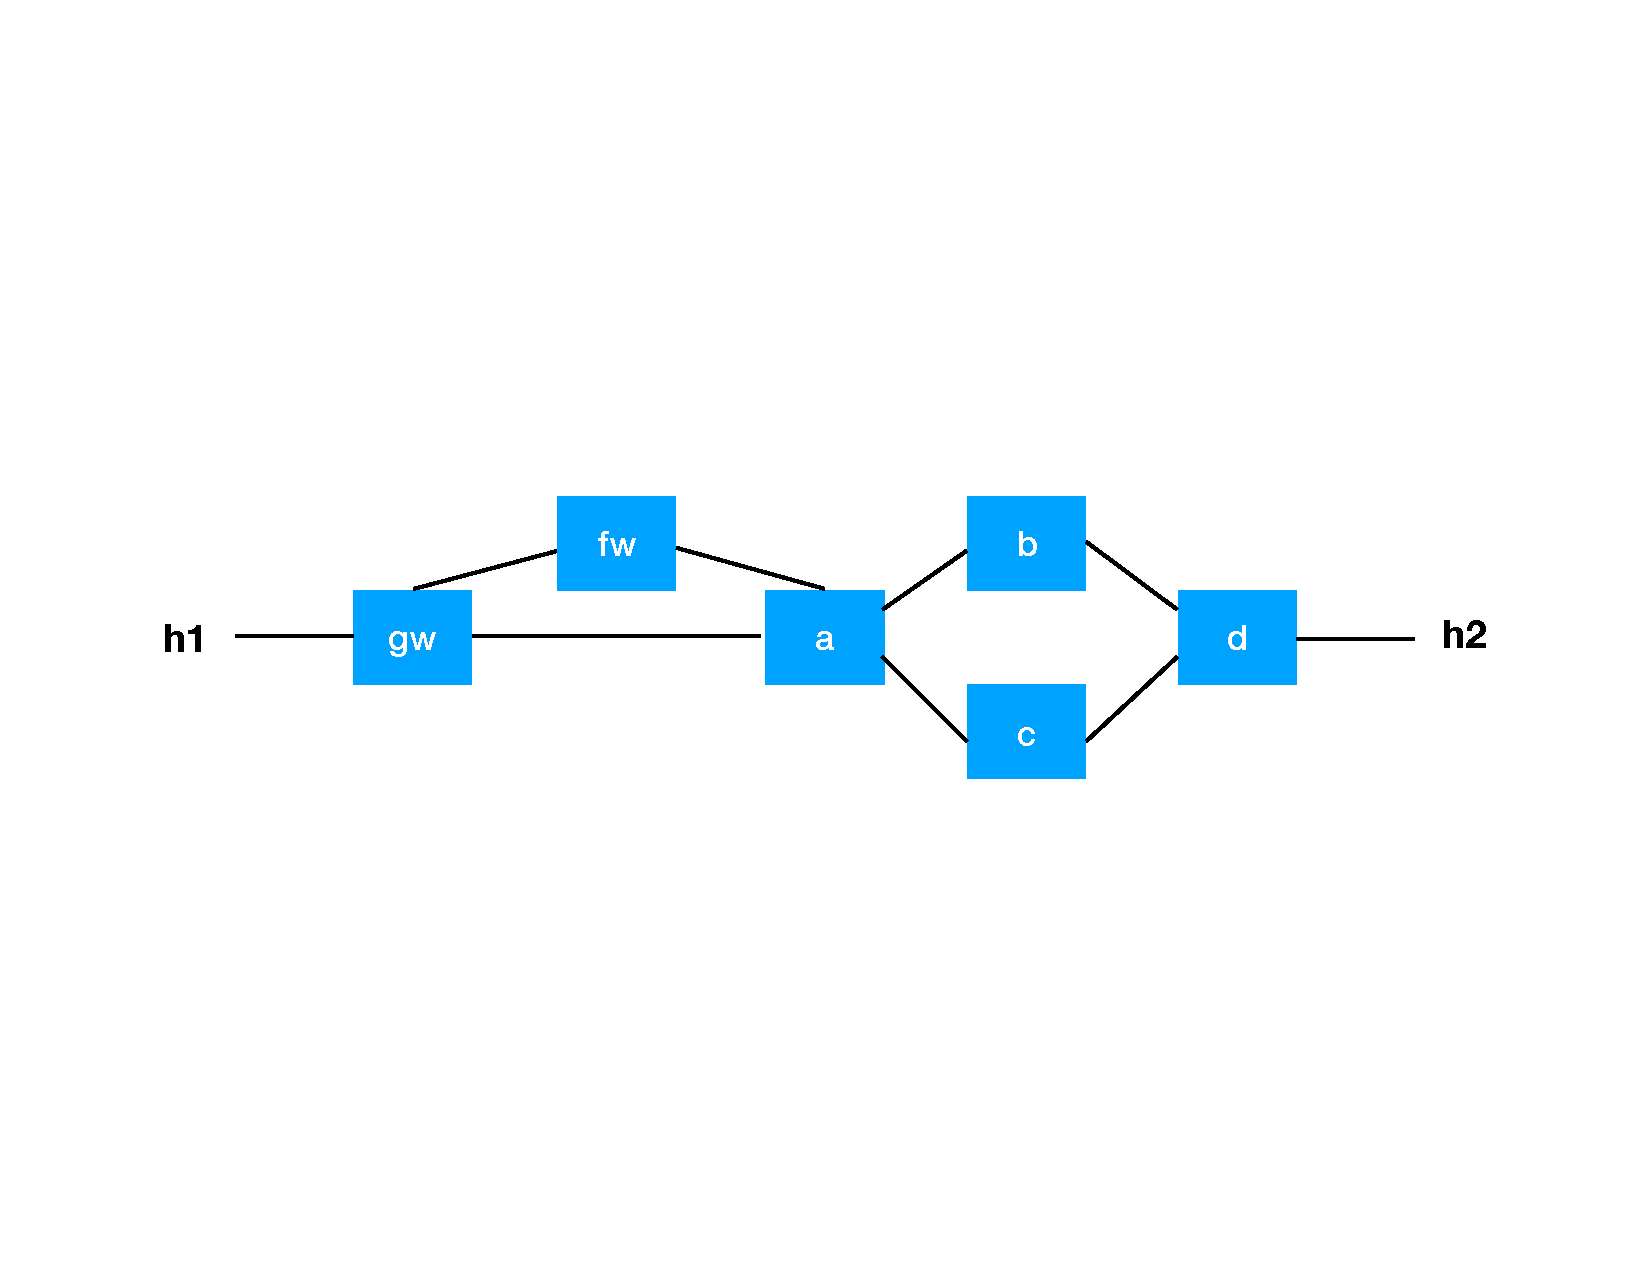
\includegraphics[width=0.8\linewidth]{figures/global-topo2.pdf}
\centering
\caption{\small 引入中间盒的网络拓扑。}
\label{fig:topo2}
\end{figure}

现在我们来看图~\ref{fig:code2}中的程序。其中L2(L3)指定了转发路径约束,即路径从$h_1$至$h_2$并需经过节点$b$ ($c$)。在返回语句中通过\emph{any}的函数(路由代数~\cite{gao2018t}),标明选出满足约束的任何一条路径。虽然编程模型非常直接简单,但由于引入中间盒对数据包的处理操作,而中间盒需要映射到网络的物理节点,系统需要保证程序的正确性。

\para{正确性}:我们采用如下对于正确性的定义:对于任何数据包$pkt$,其在网络中的真实转发路径必须要符合程序中返回的对数据包$pkt$的路径。例如,如果程序员使用\emph{opt}函数来选择一个满足约束的最少跳数路径,即\codeword{opt(PATH1)}),则真实转发路径应为网络中的$gw, a, b, d$。然而,由于数据包必须要经过防火墙,其真实转发路径必须包含防火墙$fw$,从而不符合程序中返回的路径。

为了保证正确性,一个简单的做法是让程序员显式地在路径约束上包含需要的中间盒节点。在上述场景中,其应为\codeword{PATH1 = h1 -> fw -> b -> h2}。然而,让程序员来保证路径约束和网络中真实转发的一致性的做法,会给程序员带来额外的负担。

\para{系统路径约束}:为了解决上述问题,我们引入系统路径约束(System Path Constraint,SPC)的概念。在程序中,SPC表示为一个存有路径约束的全局变量。程序中的任何一个位置计算路径时需要满足SPC中的路径约束。其直观理解是,当一个数据包经过程序时,某些程序语句会给数据包添加路径约束。考虑图~\ref{fig:code3}中添加SPC后的程序。程序中的第六行添加了一个从$h_1$到$h_2$的路径约束;第七行添加了一个必须要经过防火墙的路径约束。因此,在第七行后,SPC全局变量包含如下约束:从$h_1$到$h_2$以及经过防火墙$fw$。第八行中使用\emph{opt}函数计算路径,其中``+''表示连接SPC的路径约束和PATH1的路径约束,而其结果为$gw, fw, a, b, d$。

\begin{figure}[h]
{\small
\begin{verbatim}
L1: mFW = middlebox("firewall", "stateless")
L2: PATH1 = h1 -> b -> h2 //b: waypoint
L3: PATH2 = h1 -> c -> h2 //c: waypoint
L4: //any: picking any path
L5: def onPacket(pkt):
L6:   if pkt.srcAddr == h1 & pkt.dsrAddr == h2:
L7:     if mFW.handle(pkt) == SENSITIVE:
L8:       return opt(PATH1 + SPC)
L9:     else:
L10:      return opt(PATH2 + SPC)
L11:  else: return DROP
\end{verbatim}
}
    \caption{加入SPC的程序。}
\label{fig:code3}
\end{figure}

\para{网络实现}:在保证正确性的情况下,部分可编程网络实现问题等价于添加SPC约束后的完全网络实现问题。而SPC约束的增加只是在计算决策树中叶子节点路径时需要考虑,因此我们这里不再对部分可编程网络实现问题进行讨论。

\section{实验评估}

我们这里将对计算决策树中节点与网络交换机的对应关系中的混合整数线性规划的执行时间进行评估。评估是在16GB内存以及3.5 GHz Intel i7处理器上运行,系统为Mac OSX 10.13。


\begin{figure}[ht]
  \centering
  % \subfigure[\#P = 4, \#N = 20]{
  %   \label{fig:eval-gb:a} %% label for first subfigure
  %   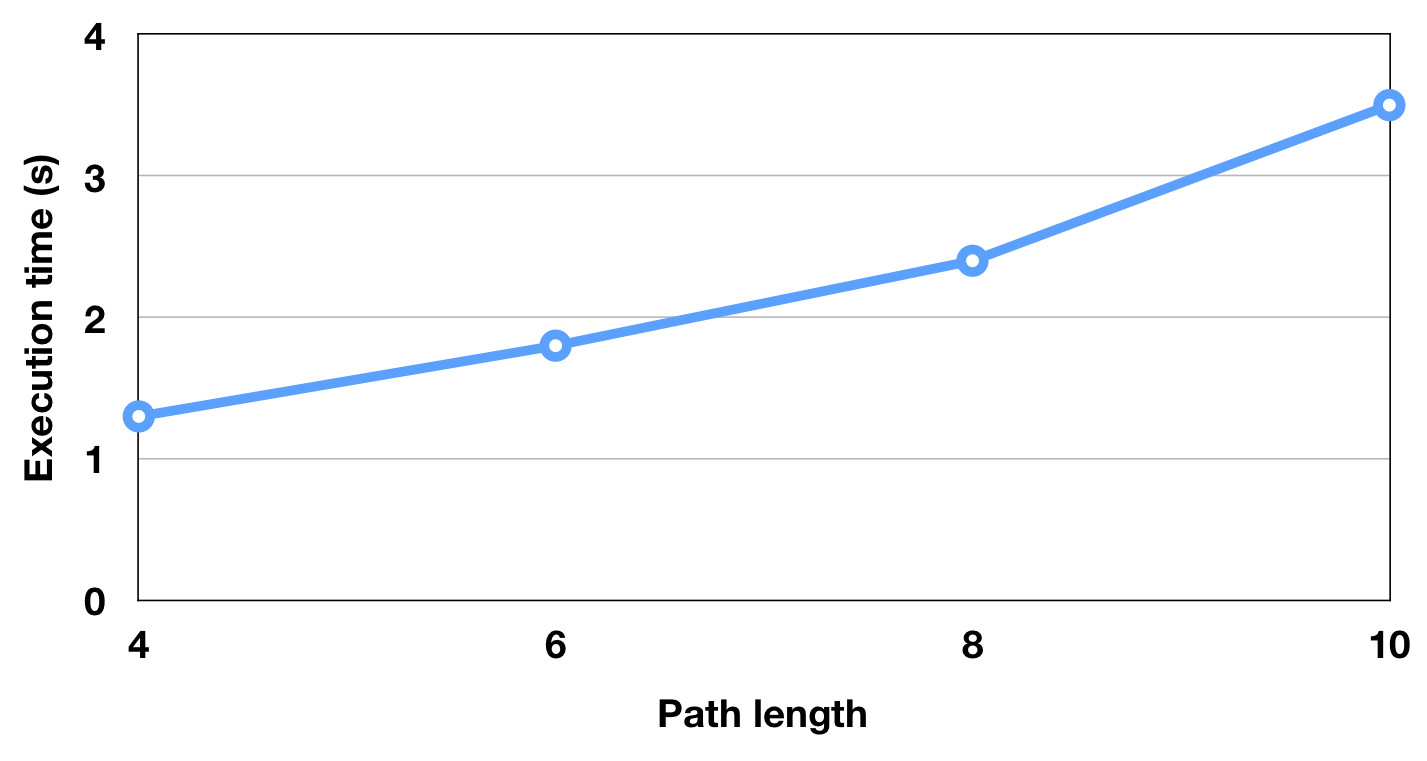
\includegraphics[width=0.4\textwidth]{figures/global-eval-420-png.png}}

  \begin{subfigure}[b]{0.47\textwidth}
      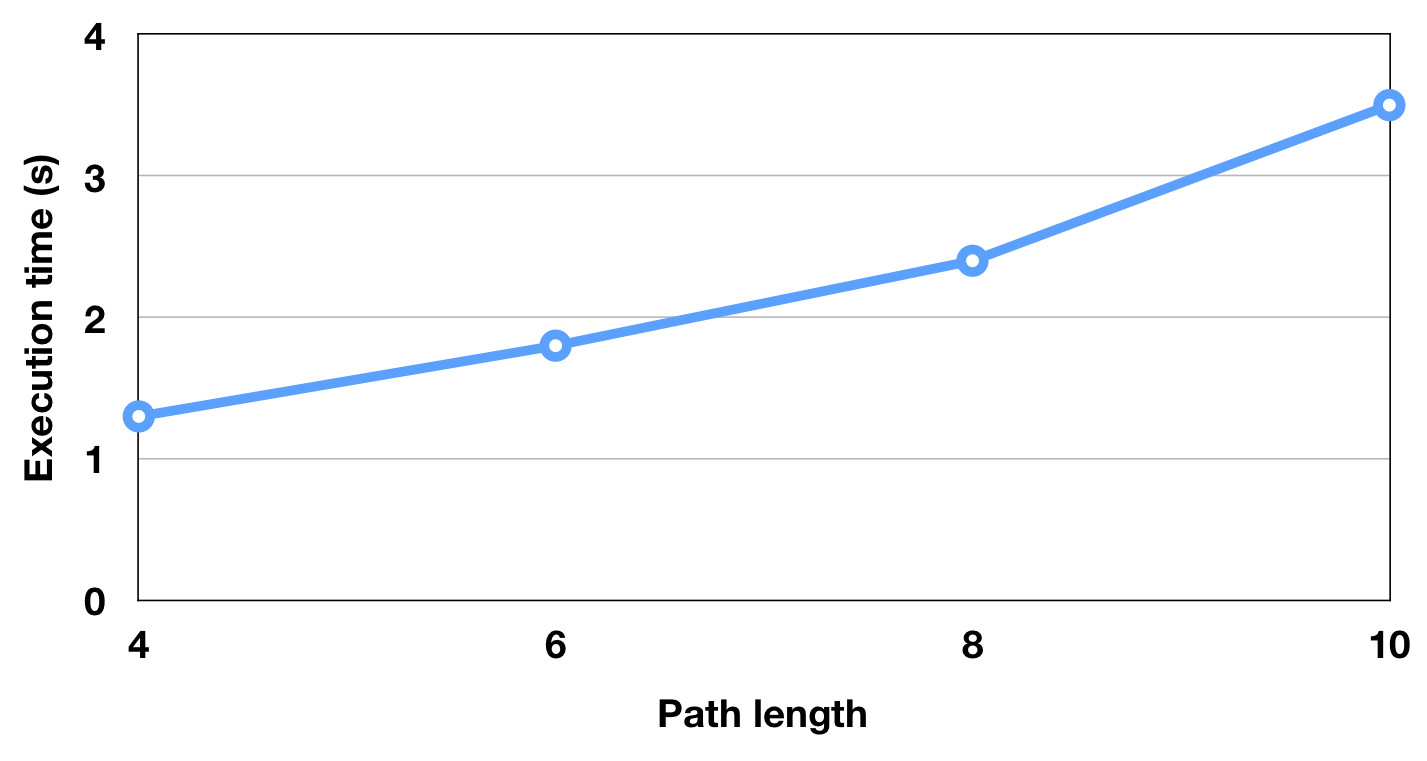
\includegraphics[width=\textwidth]{figures/global-eval-420-png.png}
      \caption{\#P = 4, \#N = 20}
      \label{fig:eval-gb:a}
  \end{subfigure}
  % \subfigure[\#P = 8, \#N = 20]{
  %   \label{fig:eval-gb:b} %% label for second subfigure
  %   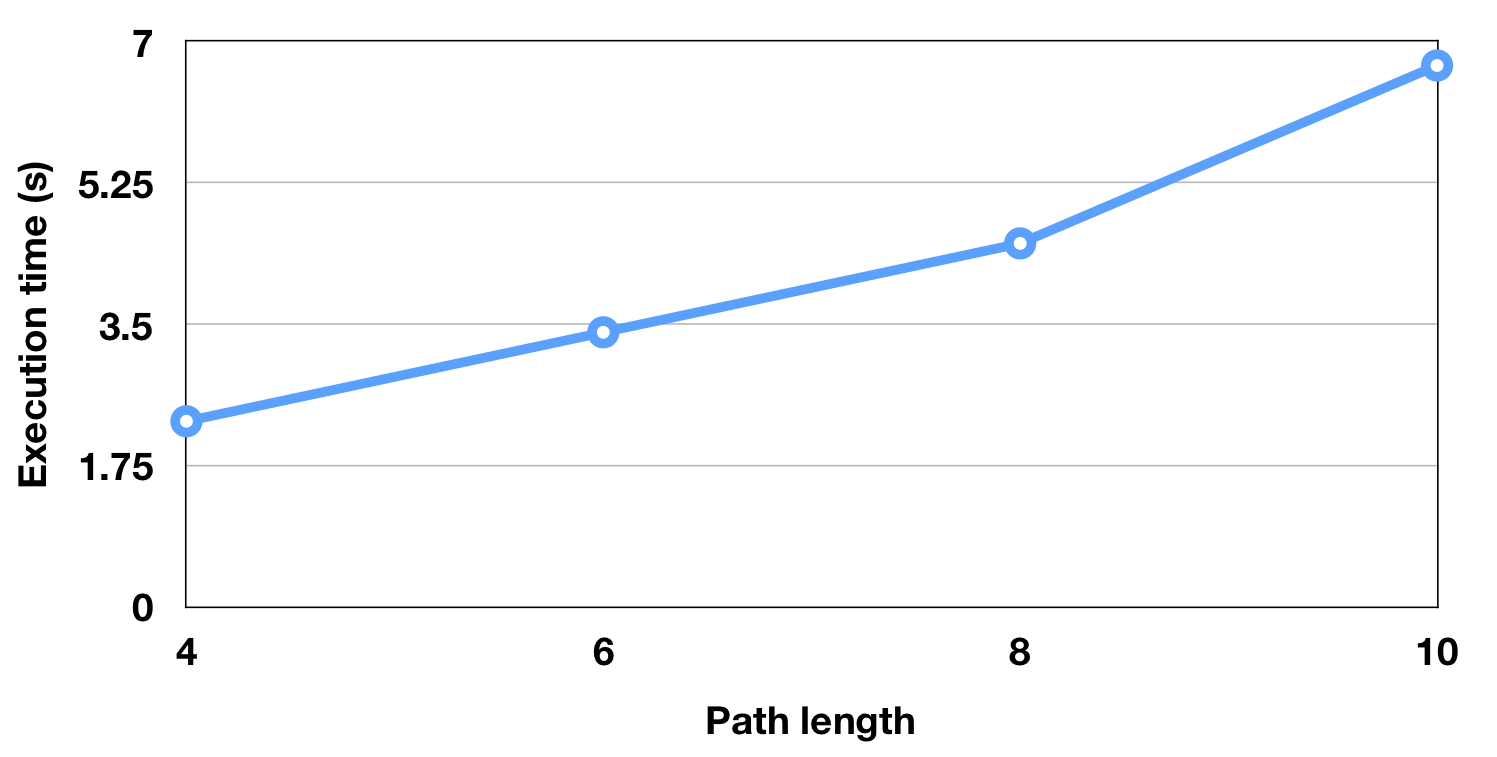
\includegraphics[width=0.4\textwidth]{figures/global-eval-820-png.png}}
  \begin{subfigure}[b]{0.47\textwidth}
      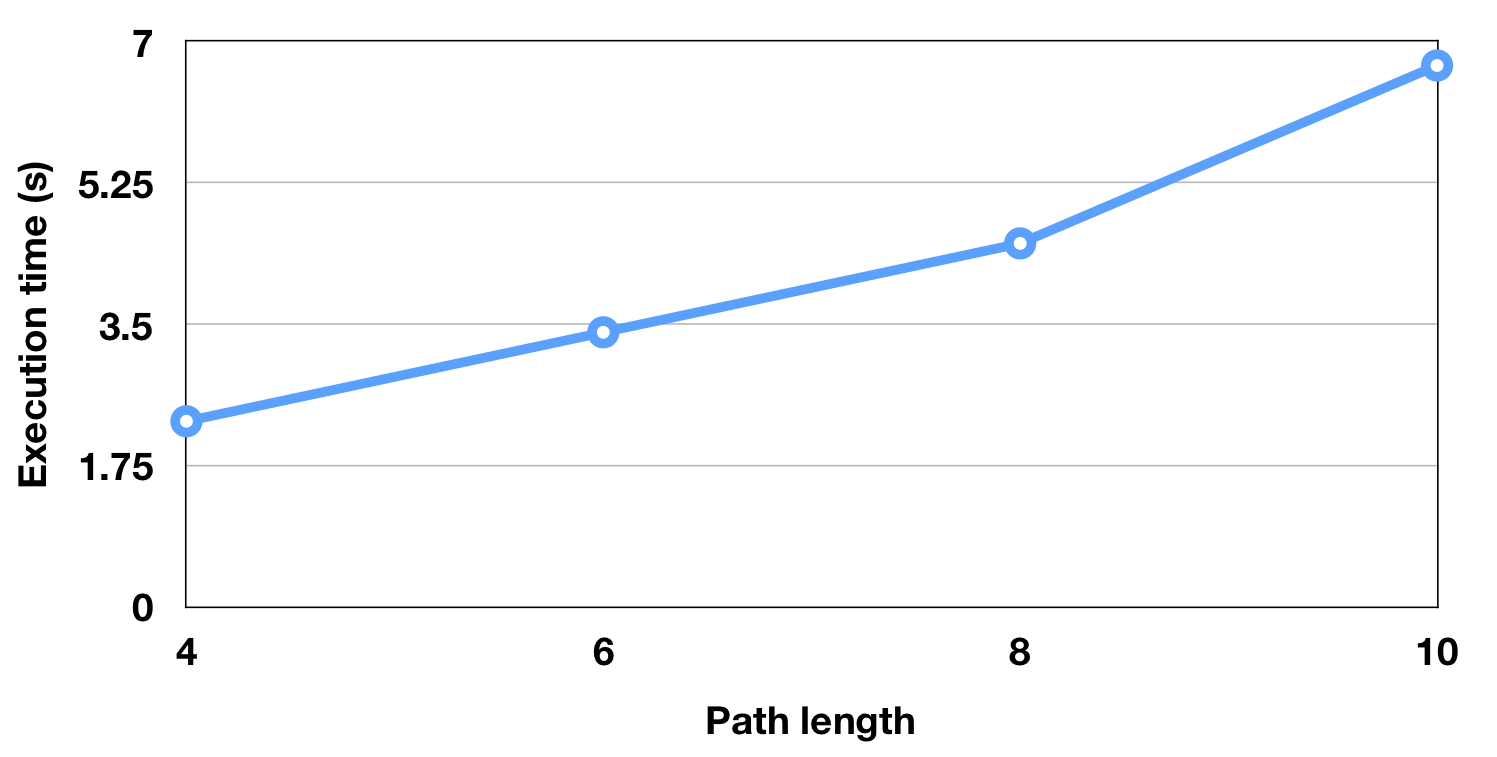
\includegraphics[width=\textwidth]{figures/global-eval-820-png.png}
      \caption{\#P = 8, \#N = 20}
      \label{fig:eval-gb:b}
  \end{subfigure}
  % \subfigure[\#P = 8, \#N = 40]{
  %   \label{fig:eval-gb:c} %% label for second subfigure
  %   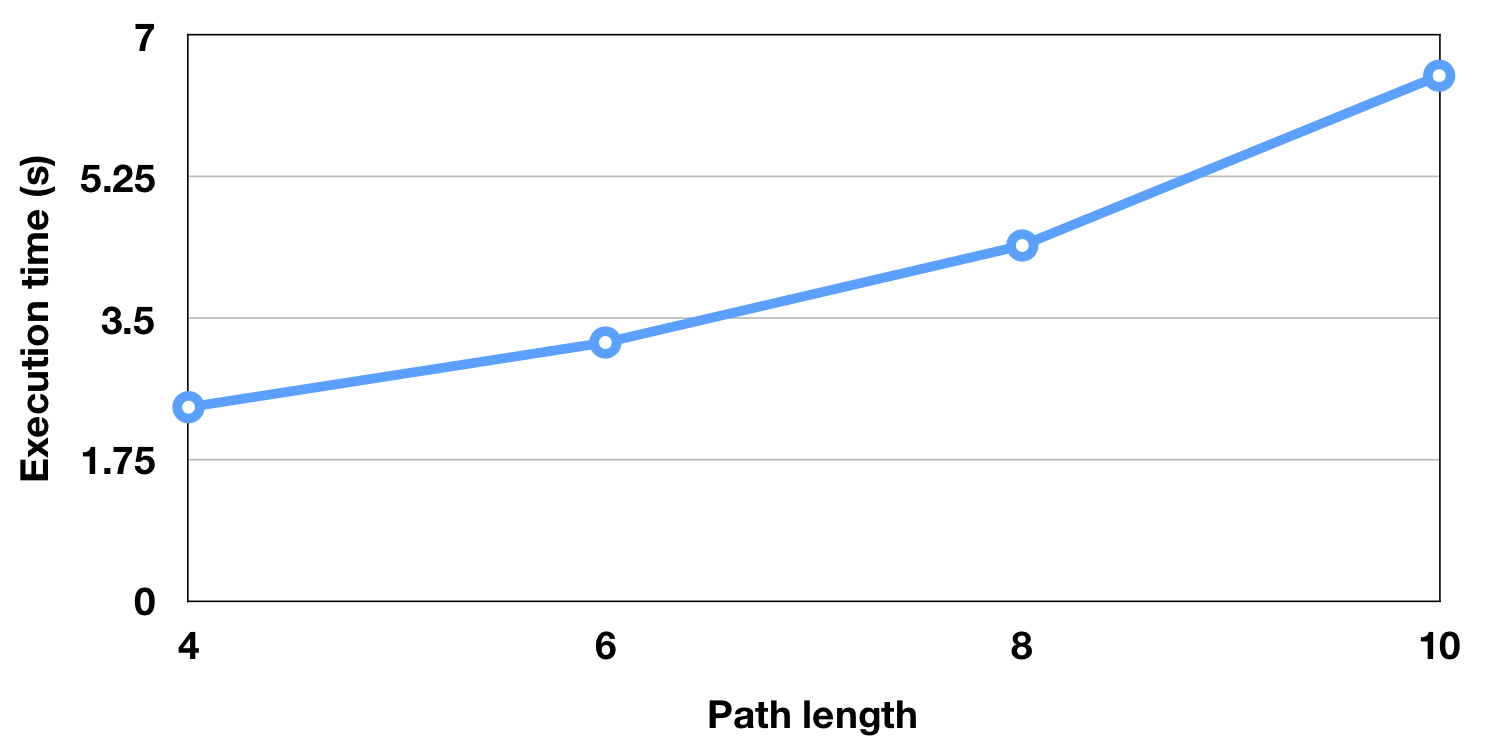
\includegraphics[width=0.4\textwidth]{figures/global-eval-840-png.png}}

  \vspace{1cm}
  \begin{subfigure}[b]{0.47\textwidth}
      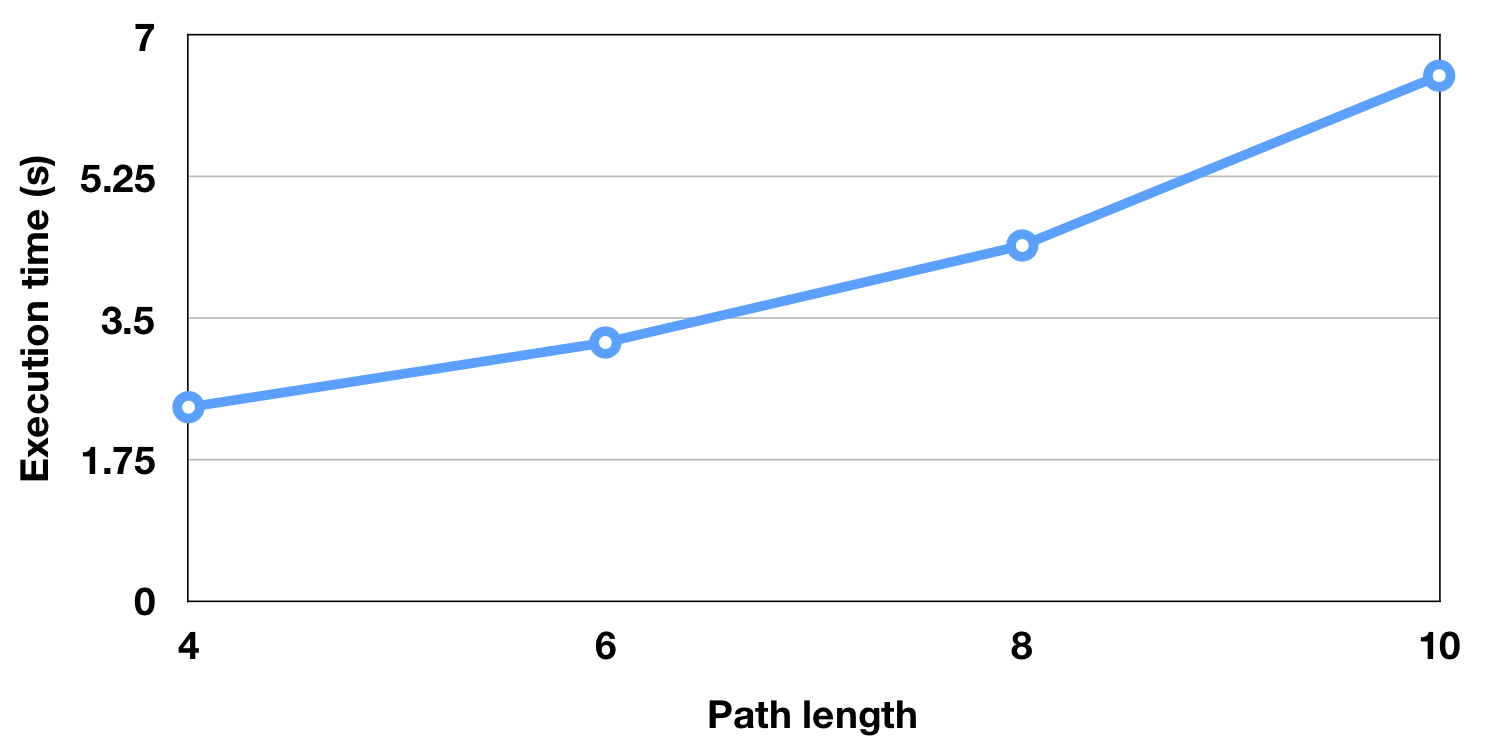
\includegraphics[width=\textwidth]{figures/global-eval-840-png.png}
      \caption{\#P = 8, \#N = 40}
      \label{fig:eval-gb:c}
  \end{subfigure}

  \caption{不同场景下的混合整数线性规划执行时间。}
  \label{fig:eval-gb} %% label for entire figure
\end{figure}



\para{实验方法}:我们假设决策树具有完美二叉树结构,并通过改变决策树的大小,对相应的叶子节点(即转发路径)的数量以及程序语句的数量进行变化。给定转发路径数量下,在随机生成的拓扑图中随机生成相应数量且满足路径长度的转发路径,并随机地填充到决策树的叶子节点中。最后根据决策树以及拓扑图计算决策树中节点与网络交换机的对应关系,并记录混合整数线性规划的执行时间。

\para{实验结果}:图~\ref{fig:eval-gb}给出在不同场景下的执行时间。其中\#P代表路径数量;\#N代表图中节点数量。从图~\ref{fig:eval-gb:a}可以看出,当路径长度增加时,混合整数线性规划的执行时间变长;通过比较图~\ref{fig:eval-gb:a}和图~\ref{fig:eval-gb:b},我们可以发现,当路径数量增加时,混合整数线性规划的执行时间变长;通过比较图~\ref{fig:eval-gb:b}和图~\ref{fig:eval-gb:c},我们可以发现,在其他变量不变情况下,拓扑的规模变大不会增长执行时间。这是因为,决策树节点的放置范围已经固定在各自所属的转发路径上,拓扑图中其他节点的增加不会影响已有决策树节点的放置范围。



\section{本章小结}

本章研究了高级灵活的SDN程序面向全网络数据平面实现问题。当网络节点全部为可编程交换机时(即完全可编程网络),提出将程序拆分并部署到不同交换机的方案,并算出给定目标下的最优部署;当网络节点存在固定功能节点时(如防火墙)(即部分可编程网络),考虑了程序正确性的问题。并提出系统路径约束的概念保证程序的正确。



